\chapter{Integer Programming}
This chapter focuses on some preliminaries around integer
programming---which is a subarea of (mathematical) optimization.
In that context we introduce three common optimization problems which
can be solved using integer programming: SAT, Vertex Cover, and
Independent Set. They will appear later on in this thesis
(\cref{cha:triangulations,cha:mmlt}) in association with the
\gls{MMLT} problem.

An integer program is basically a problem description as a system
of (in-)equations involving only variables with integer values. As
an addition there can be an objection function for modeling
optimization problems. Throughout this thesis, we assume that all
of the (in-)equations are linear which is referred to as a
\emph{linear integer program}.

\begin{definition}[(Linear) \gls{IP}]
  An \gls{IP} is a system of integer variables
  \(x \in \gls{Z}^n\) with a set of constraints on them and often an 
  objective function \(c^T x\). We consider only the case where the 
  constraints are linear: \(Ax \leq b\) or \(Ax \geq b\).
\end{definition}

A natural standardized way of formulating (linear) \gls{IP}[s] is the 
so called \emph{canonical form.} It combines the variable coefficients
for all (in-)equations in a matrix \(A\), all constant terms are
summed up to a vector \(b\), and the objective function is represented
as a multiplication of the variables \(x\) and a constant target
vector \(c\). For readability, we slightly modify the canonical form,
e.g. by allowing sums.

\begin{problem}[\gls{IP} in canonical form \cite{combinatorial_optimization}]
  \[
  \begin{array}{lll}
    \begin{alignedat}{2}
      &\text{maximize } & c^Tx \\
      &\text{subject to } & Ax &\leq b \\
      && x &\geq 0 \\
      && x &\in \gls{Z}
    \end{alignedat}
    & \text{\hspace{2em}or\hspace{2em}} &
    \begin{alignedat}{2}
      &\text{minimize } & c^Tx \\
      &\text{subject to } & Ax &\geq b \\
      && x &\leq 0 \\
      && x &\in \gls{Z}
    \end{alignedat}
  \end{array}
  \]
\end{problem}

Even though the structure of \gls{IP}[s] looks very simple, it is a
long known fact that solving them is not easy. Nevertheless the come
in handy for various optimization problems---especially because there
are many practical applications involving only integers. A common
strategy to simplify the problem is leaving out the integrity
restriction for retrieving bounds of the optimal solution.

\begin{theorem}
  Solving \gls{IP}[s] is NP-hard.
\end{theorem}

\begin{proof}
  Even the special case where there is no objective function, only
  binary variables, and only equality constraints is NP-complete
  \cite{karp_np_complete}. Therefore the more general problem is
  NP-hard.
\end{proof}

\section{SAT}
\todo[inline]{glue text}

\begin{problem}[3-SAT]
  \label{prob:3SAT}\hfill
  \begin{labeling}{\hspace{4em}}
    \item[\textbf{Given:}]
      Set of boolean literals \(x_i \in X\), a formula in conjunctive 
      normal form consisting of clauses \(c \in C\) each involving 
      exactly three literals (or their negations)
    \item[\textbf{Sought:}]
      An assignment for \(X\) which lets all clauses in \(C\) evaluate
      to ``true''
  \end{labeling}
\end{problem}

\todo[inline]{glue text}

\begin{theorem}[NP-completeness of 3-SAT]
  \Cref{prob:3SAT} is NP-complete.~\cite[Satisfiability with at most %
  3 Literals per Clause]{karp_np_complete}
\end{theorem}

\todo[inline]{glue text}

\begin{problem}[IP formulation of 3-SAT]
  \begin{alignat*}{3}
    &(\text{minimize } & 1) \\
    &\text{subject to } & \forall c \in C : &~
    & \sum\limits_{x_i \in c} x_i + \sum\limits_{\lnot x_i \in c} (1 - x_i) &= 1 \\
    && \forall x_i \in X : &~& x_i &\in \{0,1\}
  \end{alignat*}
\end{problem}

\todo[inline]{glue text}

\begin{problem}[Planar 3-SAT]
  \label{prob:planar_3SAT}
  An instance of the 3-SAT problem with literals \(X\) and
  clauses \(C\) which can be represented by a planar graph
  \(G = (V,E)\) such that
  \begin{alignat*}{1}
    V &= \{v : v \in X \cup C\} \\
    E &= \{ \{x, c\} :
      x \in X,~
      c \in C,~
      (x \in c) \lor (\lnot x \in c)
    \}
  \end{alignat*}
\end{problem}

\todo[inline]{glue text}

\begin{figure}[ht]
  \centering
  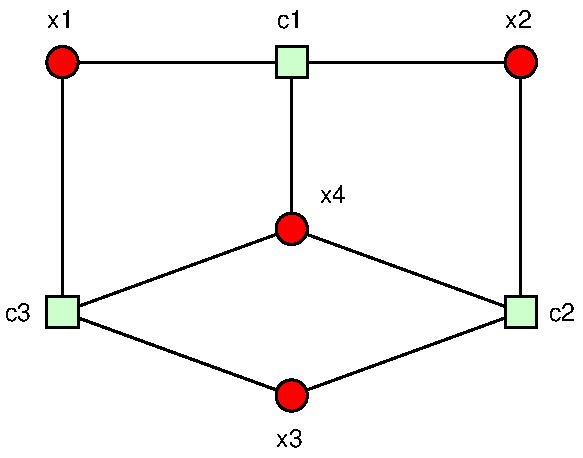
\includegraphics[width=0.5\textwidth]{img/example_planar_3SAT.pdf}
  \caption{\label{fig:example_planar_3SAT}Example of a Planar 3SAT %
    instance which represents the term \(%
      \protect\underbrace{(x_1 \lor x_2 \lor x_4)}_{c_1}\land%
      \protect\underbrace{(\lnot x_2 \lor x_3 \lor \lnot x_4)}_{c_2}\land%
      \protect\underbrace{(x_1 \lor \lnot x_3 \lor \lnot x_4)}_{c_3}%
    \)}
\end{figure}

\todo[inline]{glue text}

\begin{theorem}[NP-completeness of Planar 3-SAT]
  \Cref{prob:planar_3SAT} is still NP-complete.~\cite{planar_3SAT}
\end{theorem}

\section{Vertex Cover}
\todo[inline]{glue text}

\begin{definition}[Vertex Cover]
  \label{def:vertex_cover}
  Given an undirected graph \(G=(V,E)\), a vertex cover
  \(\gls{VC} \subseteq V\) for \(G\) is a vertex set such that
  every edge \(e \in E\) is incident to at least one vertex
  \(v \in \gls{VC}\):
  \[ \forall e \in E: \exists v \in \gls{VC}: v \in e \]
\end{definition}

\todo[inline]{glue text}

\begin{definition}[Minimal Vertex Cover]
  A vertex cover \gls{VC} for an undirected graph
  \(G=(V,E)\) is minimal if there is no vertex
  \(v \in \gls{VC}\) such that
  \(\gls{VC} \setminus \{v\}\) remains a vertex cover.
\end{definition}

\todo[inline]{glue text}

\begin{definition}[Minimum Vertex Cover]
  A vertex cover \gls{VC} for an undirected graph
  \(G=(V,E)\) is minimum if there is no other vertex cover
  \(\gls{VC}[']\) for \(G\) which has fewer vertices:
  \[
    \forall~V_{\text{cover}}'\text{ vertex cover} :
    |\gls{VC}| \leq |\gls{VC}[']|
  \]
\end{definition}

\begin{figure}[ht]
  \centering
  \begin{subfigure}{0.25\textwidth}
    \centering
    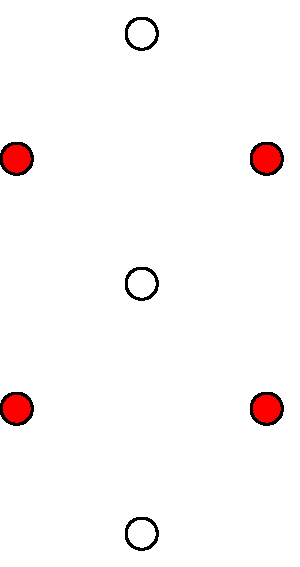
\includegraphics[width=\textwidth]{img/example_minimal_vertex_cover.pdf}
    \caption{minimal}
  \end{subfigure}
  \hspace{2em}
  \VRule
  \hspace{2em}
  \begin{subfigure}{0.25\textwidth}
    \centering
    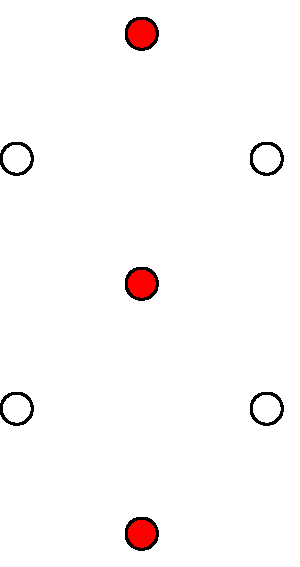
\includegraphics[width=\textwidth]{img/example_minimum_vertex_cover.pdf}
    \caption{minimum}
  \end{subfigure}
  \caption{\label{fig:example_vertex_cover}Example of minimal vs. minimum vertex cover}
\end{figure}

\todo[inline]{glue text}

\begin{problem}[\gls{IP} Formulation of Minimum Vertex Cover]
  \begin{alignat*}{3}
    &\text{minimize } & \sum\limits_{v \in V} x_v \\
    &\text{subject to } & \forall \{v,w\} \in E : &~& x_v + x_w &\geq 1 \\
    && \forall v \in V : &~& x_v &\in \{0,1\}
  \end{alignat*}
\end{problem}

\todo[inline]{glue text}

\begin{theorem}
  Vertex Cover is NP-complete. \cite{karp_np_complete}
\end{theorem}

\todo[inline]{glue text}

\begin{definition}[\Gls{wcover} Graph]
  \label{def:well_covered}
  An undirected graph \(G=(V,E)\) is \gls{wcover} iff every minimal
  vertex cover for \(G\) is also a minimum vertex cover for \(G\).
  \cite{graph_well_covered}
\end{definition}

\todo[inline]{glue text}

\begin{theorem}
  \label{thm:well_covered_vertex_cover}
  In a \gls{wcover} graph, all minimal vertex covers have the same
  cardinality. \cite{graph_well_covered}
\end{theorem}

\section{Independent Set}

\todo[inline]{glue text}

\begin{definition}[Independent Set]
  \label{def:independent_set}
  Given an undirected graph \(G=(V,E)\), an independent set
  \(\gls{IS} \subseteq V\) is a vertex set such that no two
  vertices \(v,w \in \gls{IS}\) are incident to the same edge 
  \(\{v,w\} \in E\):
  \[
    \forall v \in \gls{IS}:
    \forall \{v,w\} \in E:
    w \not\in \gls{IS}
  \]
\end{definition}

\todo[inline]{glue text}

\begin{definition}[Maximal/Maximum Independent Set]
  \label{def:max_independent_set}
  For an undirected graph \(G=(V,E)\), an independent set
  \(\gls{IS}\subseteq V\) is maximal if there is no vertex
  \(v \in V\setminus \gls{IS}\) such that
  \(\gls{IS} \cup \{v\}\) remains an independent set. It is
  maximum if there is no independent set \(\gls{IS}'\) with
  larger cardinality.
\end{definition}

\todo[inline]{glue text}

\begin{problem}[\gls{IP} Formulation of Maximum Independent Set]
  \begin{alignat*}{3}
    &\text{maximize } & \sum\limits_{v \in V} x_v \\
    &\text{subject to } & \forall \{v,w\} \in E : &~& x_v + x_w &\leq 1 \\
    && \forall v \in V : &~& x_v &\in \{0,1\}
  \end{alignat*}
\end{problem}

\todo[inline]{glue text}

\begin{theorem}[Independent Set and Vertex Cover]
  \label{thm:independent_set_vertex_cover}
  For an undirected graph \(G=(V,E)\), \(\gls{IS} \subseteq V\)
  is a maximum independent set iff
  \(\gls{VC} = V \setminus \gls{IS}\) is a minimum vertex
  cover.
\end{theorem}

\begin{proof}
  Let \gls{VC} be a vertex cover for \(G\). 
  \begin{alignat*}{1}
    \forall e \in E : \exists v \in \gls{VC} : v \in e
    &\iff \forall \{v,w\} \in E :
      v \in \gls{VC} \lor w \in \gls{VC} \\
    &\iff \forall \{v, w\} \in E :
      \lnot(v \not\in \gls{VC} \land w \not\in \gls{VC}) \\
    &\iff \forall \{v, w\} \in E :
      \lnot(v \in (V \setminus \gls{VC})
        \land w \in (V \setminus \gls{VC})) \\
    &\iff \forall v \in (V \setminus \gls{VC}) :
      \forall \{v, w\} \in E :
      w \not\in (V \setminus \gls{VC}) \\
    &\iff (V \setminus \gls{VC}) \text{ independent set}
  \end{alignat*}
  
  Assume \gls{VC} is a minimum vertex cover for \(G\) and the
  independent set \(\gls{IS} = V \setminus \gls{VC}\) is not maximum.
  Then there is an independent \(\gls{IS}['] \subseteq V\) with
  \(|\gls{IS}| < |\gls{IS}[']|\). But then for the vertex cover
  \(\gls{VC}['] = V \setminus \gls{IS}[']\) the following holds:
  \(|\gls{VC}[']| < |\gls{VC}|\)---which is a contradiction to
  \gls{VC} being minimum. The same argumentation applies in the other
  direction.
\end{proof}

\todo[inline]{glue text}

\begin{theorem}[Independent Set in \gls{wcover} Graphs]
  \label{thm:well_covered_independent_set}
  For a \gls{wcover} graph \(G=(V,E)\), every maximal independent set
  has the same size and is therefore maximum.
\end{theorem}

\begin{proof}
  \Cref{thm:well_covered_independent_set} follows directly from
  \cref{%
    def:well_covered,%
    thm:well_covered_vertex_cover,%
    thm:independent_set_vertex_cover%
  }.
\end{proof}

\todo[inline]{examples: \cref{fig:example_vertex_cover}}

\todo[inline]{glue text}

\begin{algorithm}
  \DontPrintSemicolon
  
  \KwIn{Undirected graph \(G=(V,E)\)}
  \KwOut{Maximal independent set \(\gls{IS} \subseteq V\) for \(G\)}
  
  Set \(\gls{IS} = \emptyset\) \;
  \ForEach{\(v \in V\)}{
    \If{\(\forall \{v,w\} \in E: (w \not\in \gls{IS})\)}{
        Set \(\gls{IS} = \gls{IS} \cup \{v\}\) \;
    }
  }
  \KwRet{\gls{IS}}
  \caption{\label{alg:greedy_independent_set}Greedy algorithm for independent set}
\end{algorithm}

\todo[inline]{glue text}

\begin{theorem}[Correctness and Complexity of \Cref{alg:greedy_independent_set}]
  \label{thm:greedy_independent_set}
  \Cref{alg:greedy_independent_set} always finds a maximal independent
  set in \(O(|E|)\) time.
\end{theorem}

\begin{proof}
  Because the vertices are processed sequentially, for every edge
  \(\{v,w\} \in E\) at most one of \(v\) and \(w\) is added to
  \gls{IS}. Therefore \gls{IS} is an independent set. Additionally 
  every vertex \(v \in V\) is processed and if there is no
  \(w \in \gls{IS}\) with \(\{v,w\} \in E\) then \(v \in \gls{IS}\).
  So \gls{IS} is maximal.
  
  The for-loop runs \(|V|\) times but the if-statement is only
  executed twice for every edge \(e \in E\). Every other statement
  runs in \(O(1)\) time. Thus \cref{alg:greedy_independent_set} needs
  \(O(|E|)\) time.
\end{proof}

\todo[inline]{glue text}

\begin{theorem}[\Cref{alg:greedy_independent_set} in \gls{wcover} Graphs]
  \label{thm:well_covered_maximum_independent_set}
  For a \gls{wcover} graph \cref{alg:greedy_independent_set} always
  finds a maximum independent set in \(O(|E|)\) time.
\end{theorem}

\begin{proof}
  \Cref{thm:well_covered_maximum_independent_set} follows directly
  from \cref{thm:well_covered_independent_set,thm:greedy_independent_set}.
\end{proof}

% \section{Set Cover}
% \ldots\todo[inline]{evaluate if we really need set cover}

% In the next recess Greg and his friends were discussing again what
% to play. It was always hard to find games that everybody liked.
% For example, Greg likes to play tables tennis or Duck, Duck, Goose but
% does not want to play soccer. Suddenly Greg had an idea: What about
% making a list of everybody's first and second choice and then 
% finding groups which could play together. His friends agree and
% you can see the result in \cref{tab:game_voting}.
% 
% \begin{table}[ht]
%   \centering
%   \begin{tabular}{l|cccc}
%     & table tennis & Duck, Duck, Goose & soccer & swings \\
%     \hline
%     Greg  & 1 &   &   & 2 \\
%     Joey  & 2 & 1 &   &   \\
%     Susan & 1 &   & 2 &   \\
%     Bella &   &   & 2 & 1 \\
%     Jenny & 1 & 2 &   &   \\
%     Jason &   &   & 1 & 2 \\
%     Alice &   & 2 &   & 1 \\
%     Bob   &   & 1 & 2 &   \\
%   \end{tabular}
%   \caption{\label{tab:game_voting}Voting of Greg and his friends}
% \end{table}

% Then Greg went to Mrs. Lloyd and asked her how they could find the 
% best solution. Firstly, she made another list
% (\cref{tab:example_set_cover}) where she put all the children's
% names for each game and summed up their preferences.%
% \footnote{Note that I cheated here: Usually you would divide the
% sum of preferences by the number of children who want to play the
% game. But Greg did not know yet how to divide, so I made all the
% groups have equal size.}

% \begin{table}[ht]
%   \centering
%   \begin{tabular}{lc}
%     table tennis (Greg, Joey, Susan, Jenny): & 4 \\
%     Duck, Duck, Goose (Joey, Jenny, Alice, Bob): & 6 \\
%     soccer (Susan, Bella, Jason, Bob):       & 7 \\
%     swings (Greg, Bella, Jason, Alice):      & 6 \\
%   \end{tabular}
%   \caption{\label{tab:example_set_cover}Summed up preferences for each game}
% \end{table}

% Mrs. Lloyd showed the children that there were no two games to cover
% all of them --- so they needed to split up into at least three groups.
% The best way to do so was to play table tennis, Duck, Duck, Goose, and
% on the swings. That was everybody's first choice besides for Jason.
% The problem Mrs. Lloyd solved is an instance of the minimum weight 
% set cover problem.

% \begin{problem}[Minimum Weight Set Cover]\label{prob:mwsc}
%   \hfill
%   \begin{labeling}{\hspace{4em}}
%     \item[\textbf{Given:}]
%       A ``universe'' (set) of objects \(U\), 
%       subsets \(S = \{S_i\}\)
%       such that \(\bigcup\limits_{S_i \in S} S_i = U\),
%       and a weight function \(c : S \to \gls{R}_+\)
%     \item[\textbf{Sought:}]
%       A set \(R \subseteq S\)
%       which covers the universe, i.e. 
%       \(\bigcup\limits_{S_i \in R} S_i = U\)
%       and minimizes \(\sum\limits_{S_i \in R} c(S_i)\)
%   \end{labeling}
% \end{problem}
% 
% \Cref{prob:mwsc} is NP-hard \cite{set_cover} and the related decision 
% problem was already one of the problems Karp has shown to be 
% NP-complete \cite{karp_np_complete}.

%---------------------------------------------------------------------##########
